\documentclass[12pt,a4paper]{article}
\usepackage{ctex}
\usepackage{amsmath,amscd,amsbsy,amssymb,latexsym,url,bm,amsthm}
\usepackage{epsfig,graphicx,subfigure}
\usepackage{enumitem,balance}
\usepackage{wrapfig}
\usepackage{mathrsfs, euscript}
\usepackage[usenames]{xcolor}
\usepackage{hyperref}
\usepackage[vlined,ruled,commentsnumbered,linesnumbered]{algorithm2e}
\usepackage{float}
\usepackage{array}
\usepackage{diagbox}
\usepackage{color}
\usepackage{indentfirst}
\usepackage{fancyhdr}
\usepackage{gensymb}
\usepackage{geometry}
\usepackage{setspace}
\usepackage{aurical}
\usepackage{times}
\usepackage{caption}
\usepackage{fontspec}
\usepackage{booktabs}
\usepackage{listings}
\usepackage{xcolor}
\setmainfont{Times New Roman}

\newtheorem{theorem}{Theorem}[section]
\newtheorem{lemma}[theorem]{Lemma}
\newtheorem{proposition}[theorem]{Proposition}
\newtheorem{corollary}[theorem]{Corollary}
\newtheorem{exercise}{Exercise}[section]
\newtheorem*{solution}{Solution}
\theoremstyle{definition}

\newcommand{\tabincell}[2]{\begin{tabular}{@{}#1@{}}#2\end{tabular}}
\newcommand{\postscript}[2]
 {\setlength{\epsfxsize}{#2\hsize}
  \centerline{\epsfbox{#1}}}

\renewcommand{\baselinestretch}{1.05}

\setlength{\oddsidemargin}{-0.365in}
\setlength{\evensidemargin}{-0.365in}
\setlength{\topmargin}{-0.3in}
\setlength{\headheight}{0in}
\setlength{\headsep}{0in}
\setlength{\textheight}{10.1in}
\setlength{\textwidth}{7in}
\makeatletter \renewenvironment{proof}[1][Proof] {\par\pushQED{\qed}\normalfont\topsep6\p@\@plus6\p@\relax\trivlist\item[\hskip\labelsep\bfseries#1\@addpunct{.}]\ignorespaces}{\popQED\endtrivlist\@endpefalse} \makeatother
\makeatletter
\renewenvironment{solution}[1][Solution] {\par\pushQED{\qed}\normalfont\topsep6\p@\@plus6\p@\relax\trivlist\item[\hskip\labelsep\bfseries#1\@addpunct{.}]\ignorespaces}{\popQED\endtrivlist\@endpefalse} \makeatother

\begin{document}

\section{引言}

近年来,人们逐渐从信息化时代迈向了数据时代,各种数据爆炸式地增长,数据消费也在日益增多,大量的信息、知识和利润隐藏在这些数据中。如何更有效地利用这些数据,已经成为这个时代下人们共同探索的问题之一。

\vspace{0.01\linewidth}
在这次大作业中,我将对Adult数据集进行全面的分析:首先探索数据集中各特征的分布信息;再划分数据集,尝试多种分类模型;最后比较这些模型在Adult数据集上的预测结果(分析代码均基于Python语言,相关工具和库包可参见附录 \ref{apd:tools})\footnote{本次大作业以及以往小作业的代码可参见我的github仓库:\href{https://github.com/shinshiner/CS245-Data-Science}{https://github.com/shinshiner/CS245-Data-Science}}。

\section{探索Adult数据集}

\subsection{Adult数据集的基本信息}

%\vspace{0.01\linewidth}
Adult数据集 \cite{Dataset} 也称人口普查收入(Census Income)数据集,来源于美国1994年的人口普查数据库,可以作为二分类数据集,用来预测居民年收入是否超过50K\$,其基本信息可参见表 \ref{tab:basic-info}。

%\vspace{0.01\linewidth}
\begin{table}[H]
	\renewcommand\arraystretch{1.35}
	\caption{Adult数据集的基本信息}
	\label{tab:basic-info}
	\centering
	
	\begin{tabular}{c|c||c|c}
		\centering
		属性 & 值 & 属性 & 值 \\
		\hline
		\hline
		数据集特征 & 多变量 & 相关应用 & 分类 \\
		实例数 & 48842 & 捐赠日期 & 1996.5.1 \\
		领域 & 社会 & 是否有缺失值 & 有 \\
		属性特征 & 类别型或整数 & 官网访问次数 & 1188850 \\
		属性数目 & 14 & & \\
		
	\end{tabular}
\end{table}

\vspace{-0.01\linewidth}
Adult数据集的每个实例包含14个属性,其含义、数据类型、取值范围等基本信息见表 \ref{tab:feature-info}。

\begin{table}[H]
	\renewcommand\arraystretch{1.15}
	\caption{Adult数据集的基本信息}
	\label{tab:feature-info}
	\centering
	
	\begin{tabular}{c|c|c|c}
		\centering
		 特征名 & 含义 & 数据类型 & 类别数 \\
		\hline
		\hline
		age & 年龄 & 整数 & - \\
		workclass & 工作类型 & 类别型 & 8 \\
		fnlwgt & 序号 & 整数 & - \\
		education & 教育程度 & 类别型 & 16 \\
		education-num & 受教育时间 & 整数 & - \\
		marital-status & 婚姻状况 & 类别型 & 7 \\
		occupation & 职业 & 类别型 & 14 \\
		relationship & 家庭关系 & 类别型 & 6 \\
		race & 种族 & 类别型 & 5 \\
		sex & 性别 & 类别型 & 2 \\
		capital-gain & 资本收益 & 整数 & - \\
		capital-loss & 	资本损失 & 整数 & - \\
		hours-per-week & 每周工作小时数 & 整数 & - \\
		native-country & 原籍 & 类别型 & 41 \\
		
	\end{tabular}
\end{table}

\subsection{数据预处理}

\vspace{0.01\linewidth}
我首先使用pandas库读取Adult数据集,将其存储为pandas库中的DataFrame格式,随机打印出其中几个实例,对该数据集进行初步的观察,结果如下。

\vspace{0.015\linewidth}
	\begin{lstlisting}[
	numbers=left,
	keywordstyle=\color{blue!70},
	frame=shadowbox,
	breaklines=True]
 age work_class  fnlwgt   education  education_num     marital_status
  24    Private  269799   Assoc-voc             11       Never-married   
  35          ?  169809   Bachelors             13  Married-civ-spouse   
  51    Private  257126        10th              6  Married-civ-spouse   
  72    Private  107814     Masters             14       Never-married   
  33    Private  205950     HS-grad              9       Never-married   

      occupation    relationship    race    sex  capital_gain
 Exec-managerial   Not-in-family   White   Male             0   
               ?         Husband   White   Male             0   
    Craft-repair         Husband   White   Male             0   
  Prof-specialty   Not-in-family   White   Male          2329   
   Other-service       Own-child   White   Male             0   

 capital_loss  hours_per_week  native_country   income  
            0              40   United-States   <=50K.  
            0              20   United-States    <=50K
            0              40   United-States   <=50K.  
            0              60   United-States    <=50K  
            0              40   United-States    <=50K   
	\end{lstlisting}
	
\vspace{0.02\linewidth}
从以上的初步观察可以得知,Adult数据集存在数据缺失的情况(如第3行和10行的“?”),我对整个数据集进行统计后,发现数据集中共有3620个实例存在缺失值,而其中2799个实例的缺失值多于1个(表 \ref{tab:nan})。同时,我发现分类目标(income)的部分值存在歧义,“<=50K.”与“<=50K”属于同类,却被赋上不同标签,在后续预处理过程中(\ref{sec:fix-target}小节)我会进行处理。

\begin{table}[H]
	\renewcommand\arraystretch{1.35}
	\caption{Adult数据集缺失值分布}
	\label{tab:nan}
	\centering
	
	\begin{tabular}{c|c|c|c|c}
		\centering
		 & 无缺失值 & 缺失1个特征 & 缺失2个特征 & 缺失3个特征 \\
		\hline

		实例数 & 45222 & 821 & 2753 & 46 \\

	\end{tabular}
\end{table}

\vspace{0.01\linewidth}
考虑到数据集中存在缺失值的实例数较少(仅占总数的7.41\%),且缺失的均为类别型变量,若用一般的方式填补会带来较大的偏差,因此我选择将这些实例直接删除,清理缺失值后的Adult数据集包含45222个实例,虽然由于删除数据导致workclass特征减少了一类(Never-worked),但相应的实例只有10个,可以忽略不计。

\subsection{Adult数据集中各特征的分布}

对Adult数据集进行检查和清理后,我开始探索Adult数据集中各特征的分布,我将数值型特征和类别型特征分别处理:对于数值型特征,我主要关注其数字特征(如均值,方差等)及分布密度;对于类别型特征,我主要关注其具体的分布情况。

\subsubsection{数值型特征的分布}
\label{sec:num_feature}

Adult数据集中的数值型特征为:age, fnlwgt, education-num, capital-gain, capital-loss以及hours-per-week。我首先统计其均值、标准差等数字特征,相应结果如表 \ref{tab:num_feature_avg}所示。

\begin{table}[H]
	\renewcommand\arraystretch{1.5}
	\caption{Adult数据集数值型特征的数字特征}
	\label{tab:num_feature_avg}
	\centering
	
	\begin{tabular}{c|c|c|c|c|c|c}
		\centering
		 特征名 &  均值 & 标准差 & 最大值 & 最小值 &  上四分位数 & 下四分位数 \\
		\hline
		\hline
		age & 38.548 & 13.218 & 90.000 & 17.000 & 47.000 & 28.000 \\
		fnlwgt & 18976.470 & 10563.920 & 1490400.000 & 13492.000 & 237926.000 & 117388.200 \\
		education-num & 10.118 & 2.553 & 16.000 & 1.000 & 13.000 & 9.000 \\
		capital-gain & 1101.430 & 7506.430 & 99999.000 & 0.000 & 0.000 & 0.000 \\
		capital-loss & 88.595 & 404.956 & 4356.000 & 0.000 & 0.000 & 0.000 \\
		hours-per-week & 40.938 & 12.008 & 99.000 & 1.000 & 45.000 & 40.000 \\

	\end{tabular}
\end{table}

上表的数据大致反映了各特征的分布情况,为更加直观地探索各数值型特征的分布趋势,我作出了相应的概率核密度分布图(高斯核),见图 \ref{fig:num_feature_dis}。

\begin{figure}[H]
	\centering
	\subfigure[age]{
		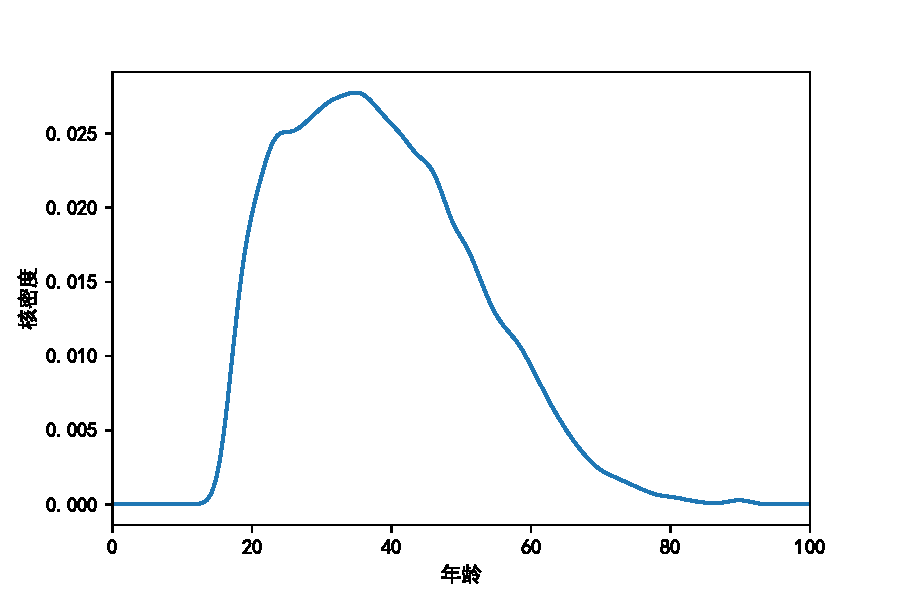
\includegraphics[width=0.31\linewidth]{img/age_dis.pdf}
	}
	\subfigure[fnlwgt]{
		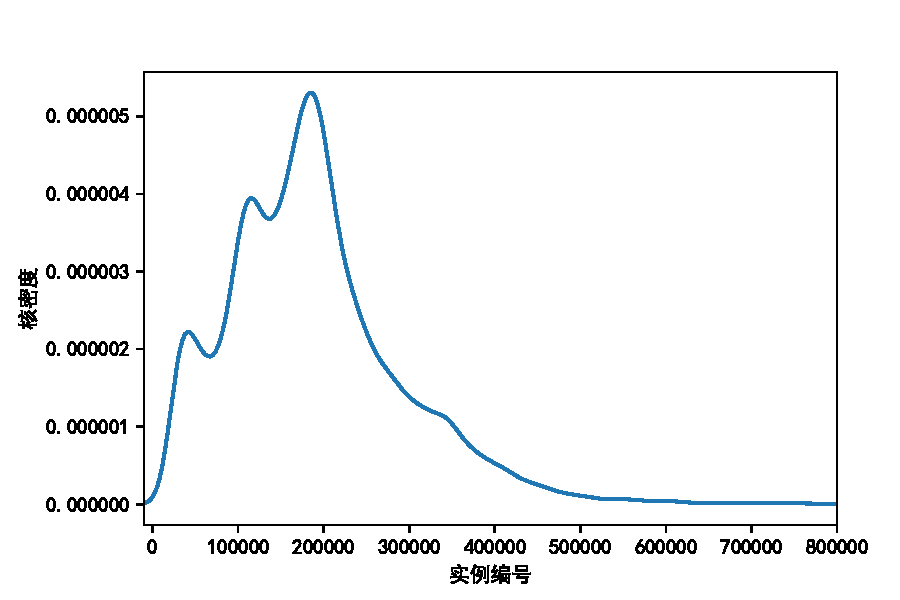
\includegraphics[width=0.31\linewidth]{img/fnlwgt_dis.pdf}
	}
	\subfigure[education-num]{
		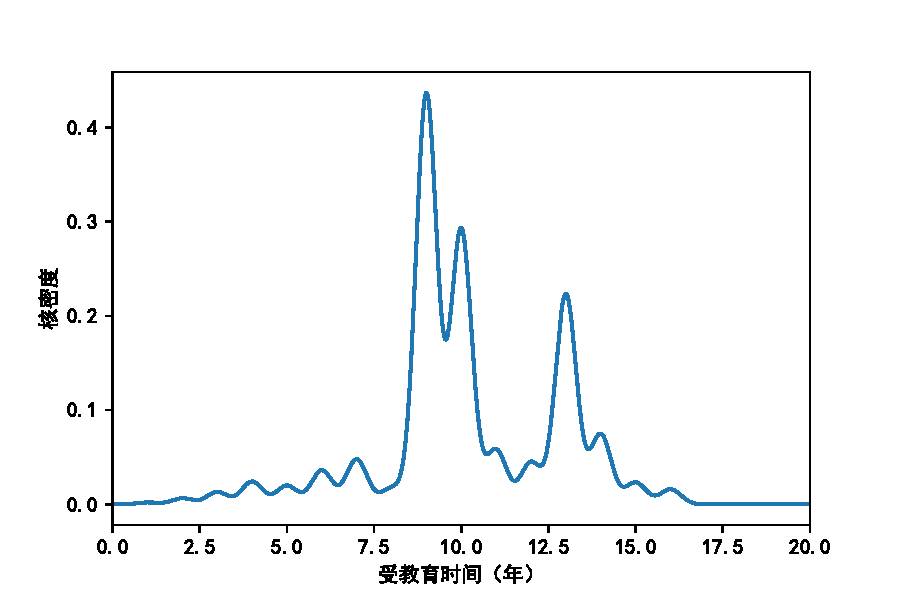
\includegraphics[width=0.31\linewidth]{img/edu_num_dis.pdf}
	}
	\subfigure[capital-gain]{
		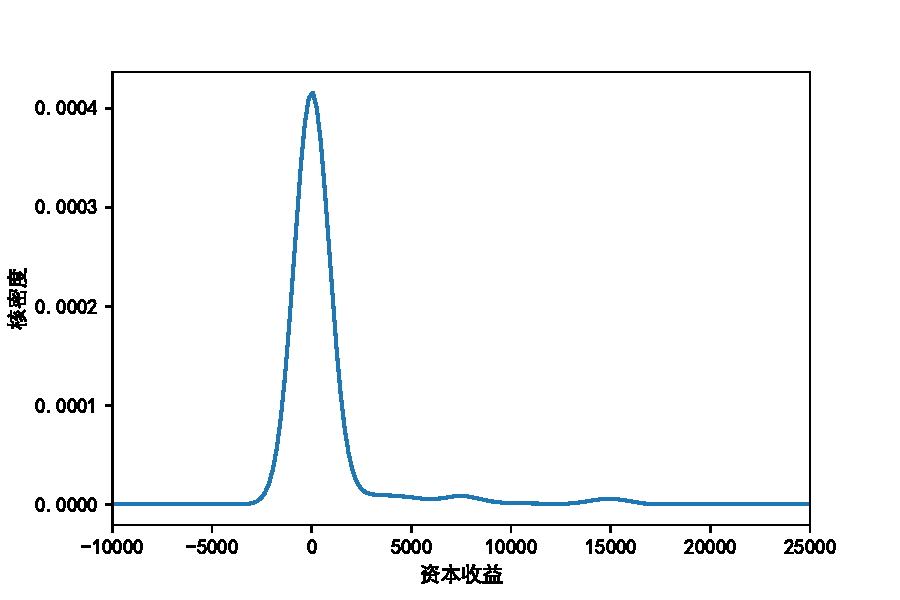
\includegraphics[width=0.31\linewidth]{img/cap_in_dis.pdf}
	}
	\subfigure[capital-loss]{
		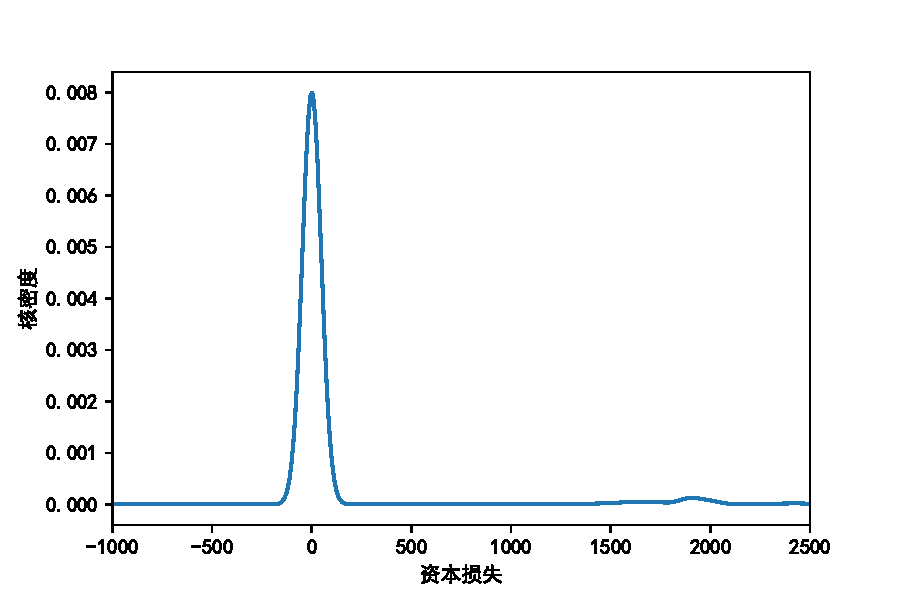
\includegraphics[width=0.31\linewidth]{img/cap_out_dis.pdf}
	}
	\subfigure[hours-per-week]{
		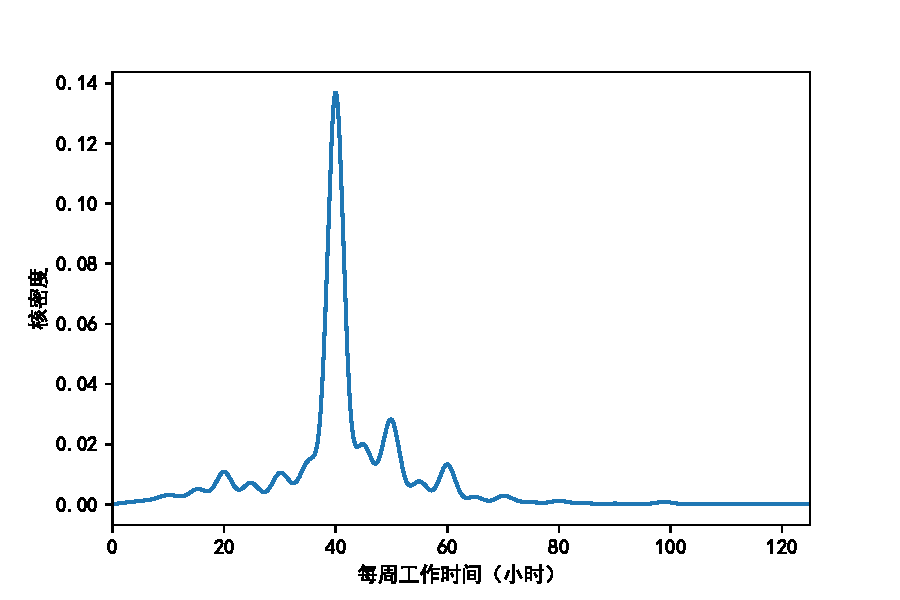
\includegraphics[width=0.31\linewidth]{img/hours_per_week_dis.pdf}
	}
	\caption{Adult数据集数值型特征概率核密度分布}
	\label{fig:num_feature_dis}
\end{figure}

\vspace{0.01\linewidth}
容易看出,Adult数据集的6个数值型特征接近于正态分布。通过进一步的观察,我发现capital-gain和capital-loss这两个特征的大部分取值均分布在0附近,仅通过概率核密度图无法了解两特征其余取值的分布情况。为更精确、详细地探索其分布,我做出了两特征对数值($log(x + 1)$)下相应的直方图(图 \ref{fig:cap-in-out})。

\begin{figure}[H]
	\centering
	\subfigure[capital-gain]{
		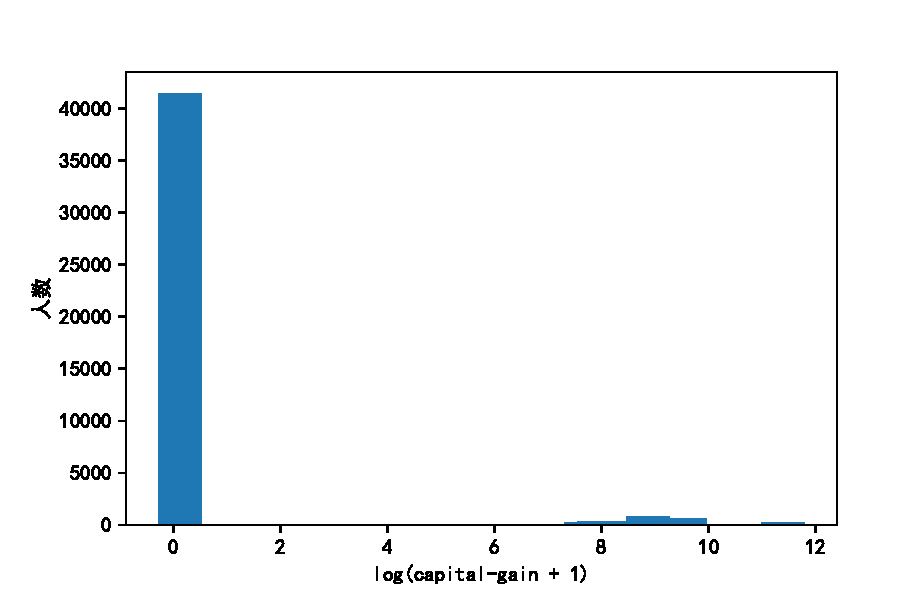
\includegraphics[width=0.41\linewidth]{img/cap-in-hist.pdf}
	}
	\subfigure[capital-loss]{
		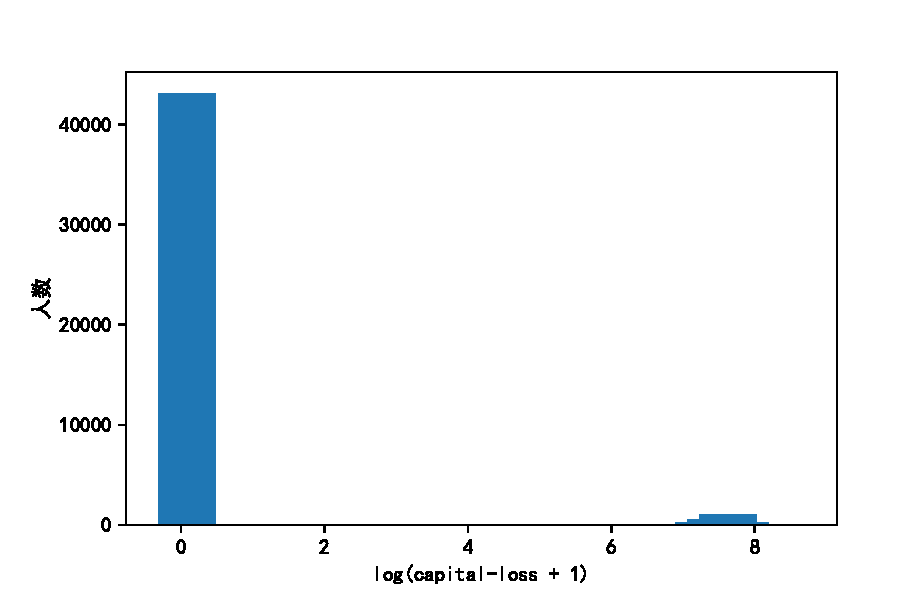
\includegraphics[width=0.41\linewidth]{img/cap-out-hist.pdf}
	}
	\caption{capital-in和capital-out的分布直方图}
	\label{fig:cap-in-out}
\end{figure}

\subsubsection{类别型特征的分布}

Adult数据集中的类别型特征包含:workclass, education, marital-status, occupation, relationship, race, sex以及native-country。我将其分布表示为条形图或饼图(图 \ref{fig:class_feature_dis1}, \ref{fig:class_feature_dis2})。各特征中包含的详细类名已记录于附录 \ref{apd:classes}中。

\begin{figure}[H]
	\centering
	\subfigure[education]{
		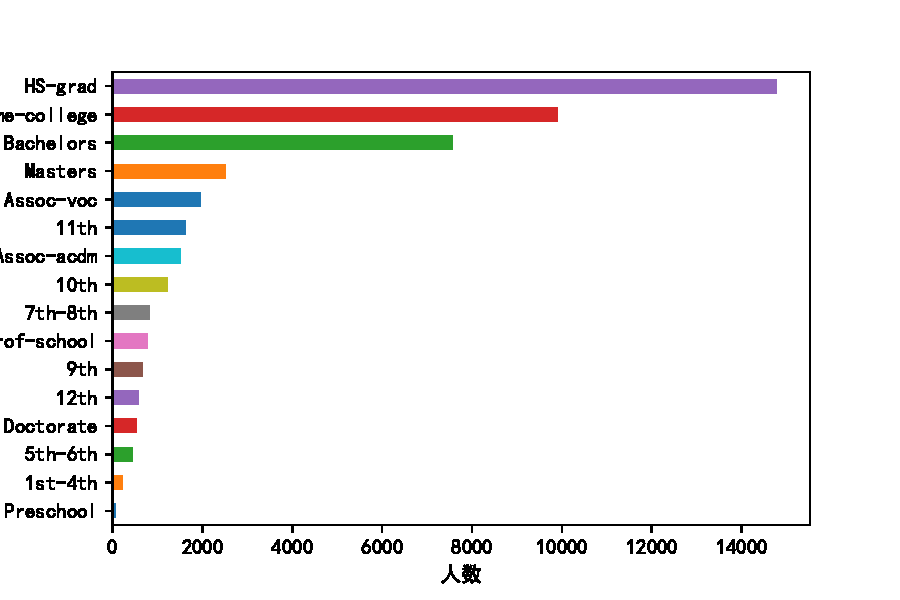
\includegraphics[width=0.43\linewidth]{img/edu_dis.pdf}
	}
	\subfigure[marital-status]{
		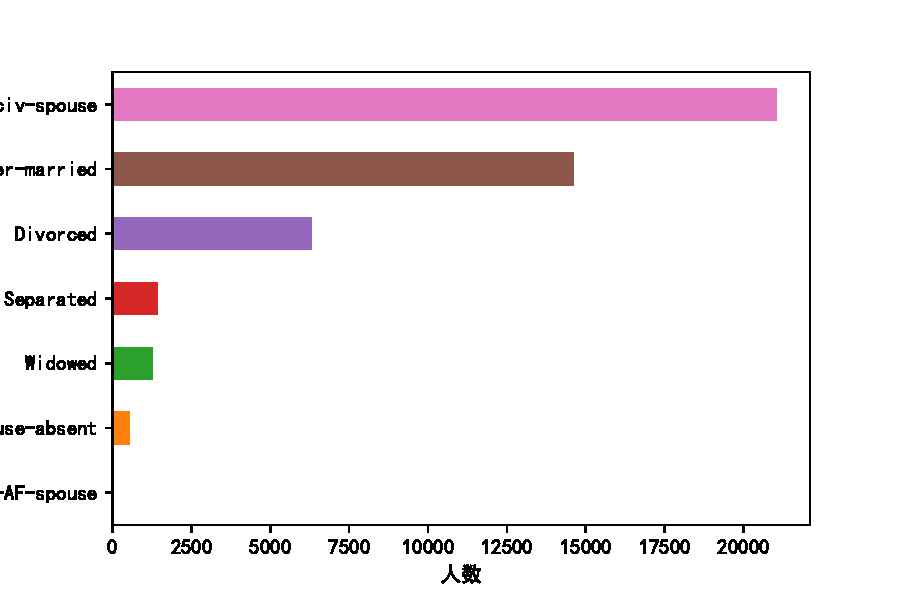
\includegraphics[width=0.43\linewidth]{img/marry_dis.pdf}
	}
	\subfigure[occupation]{
		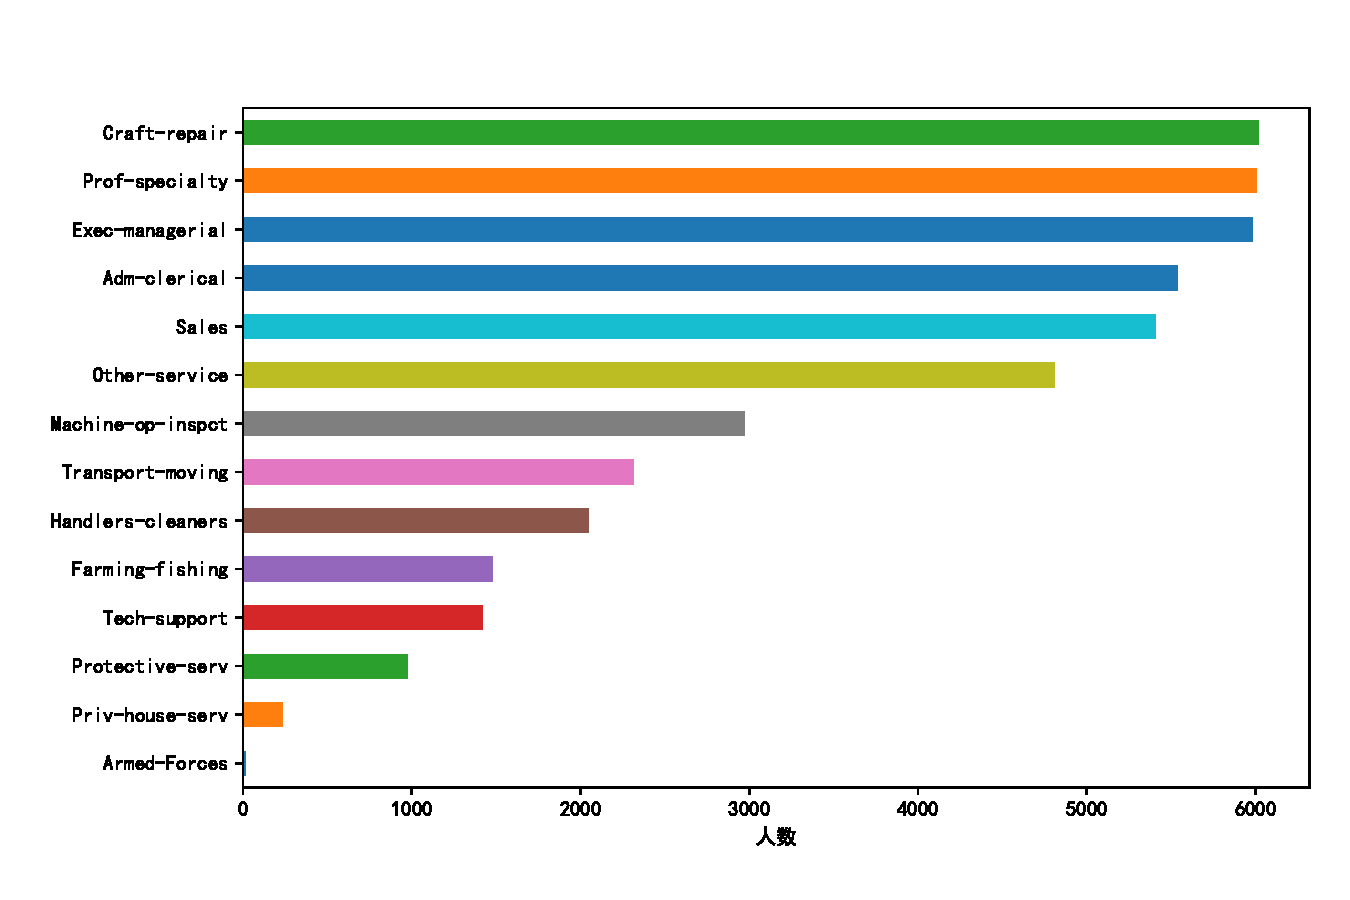
\includegraphics[width=0.43\linewidth]{img/occupation_dis.pdf}
	}
	\subfigure[race]{
		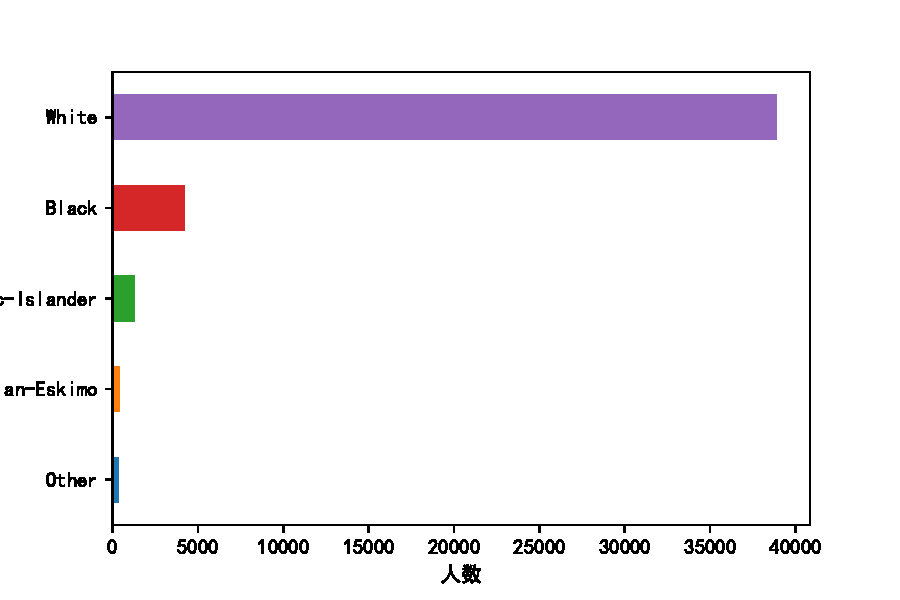
\includegraphics[width=0.43\linewidth]{img/race_dis.pdf}
	}
	\caption{Adult数据集类别型特征分布条形图}
	\label{fig:class_feature_dis1}
\end{figure}

\begin{figure}[H]
	\centering
	\subfigure[relationship]{
		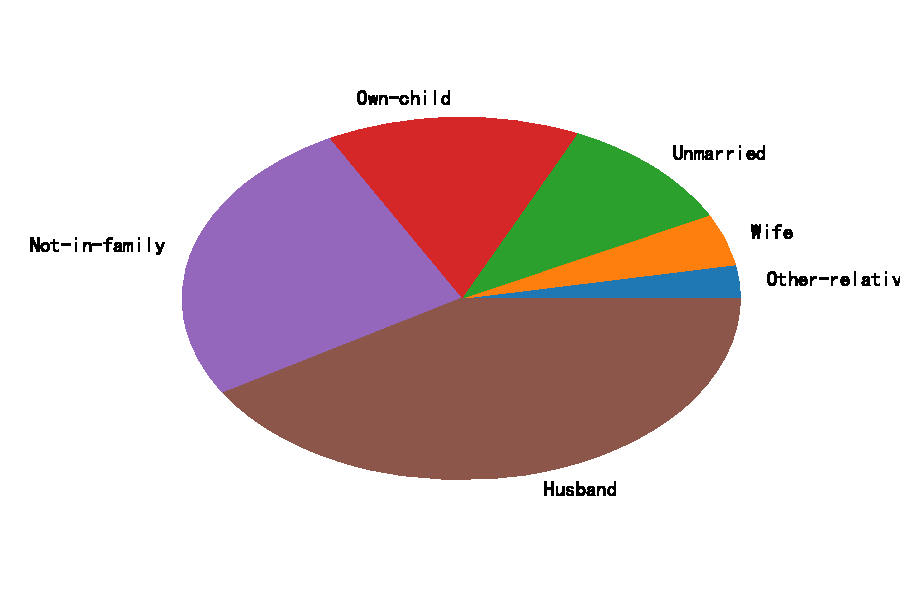
\includegraphics[width=0.43\linewidth]{img/relationship_dis.pdf}
	}
	\subfigure[sex]{
		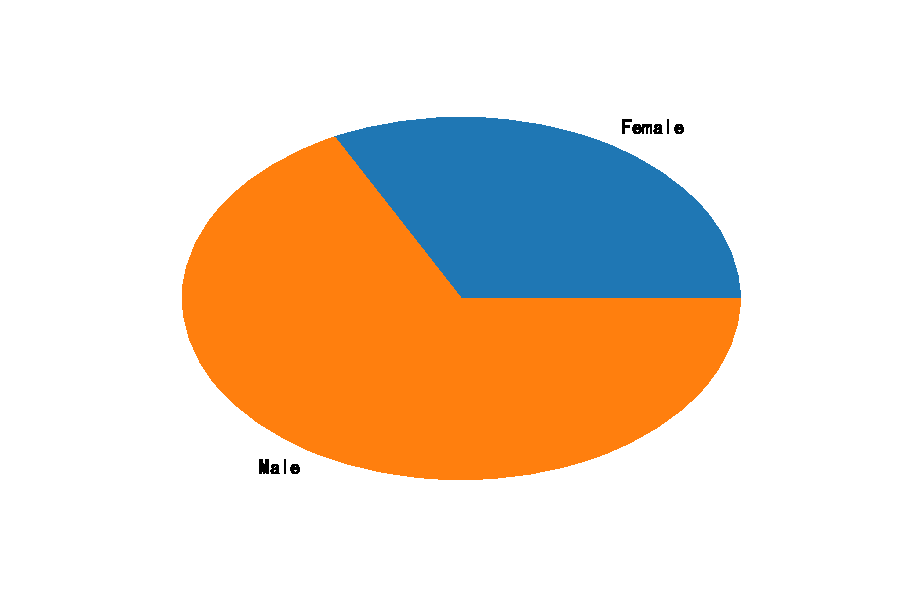
\includegraphics[width=0.43\linewidth]{img/sex_dis.pdf}
	}
	\subfigure[workclass]{
		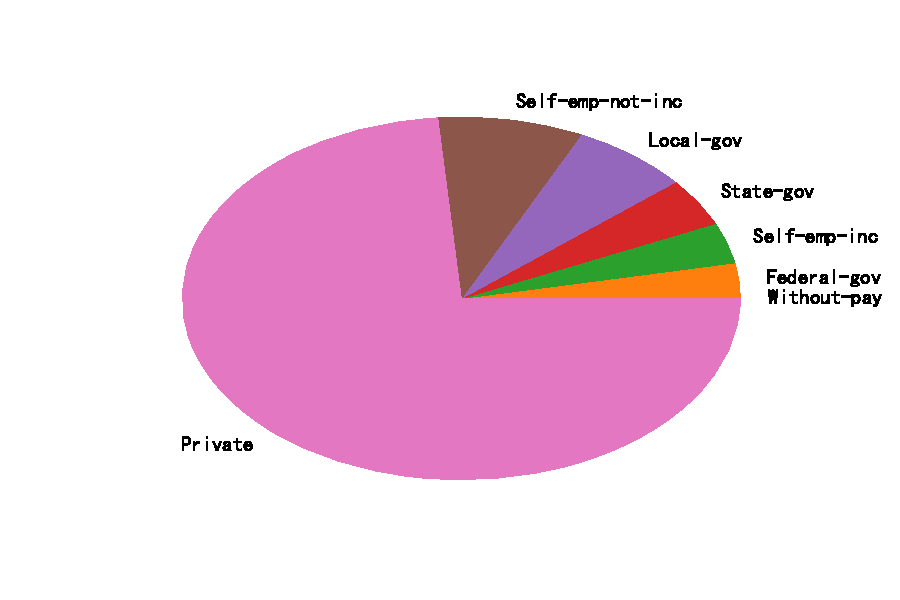
\includegraphics[width=0.43\linewidth]{img/work_class_dis.pdf}
	}
	\subfigure[workclass]{
		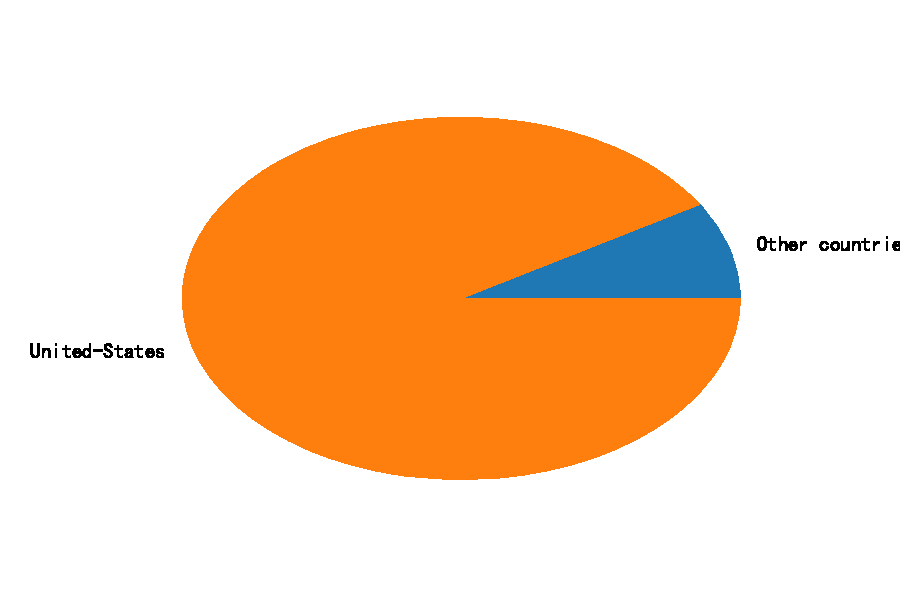
\includegraphics[width=0.43\linewidth]{img/native_country_dis.pdf}
	}
	\caption{Adult数据集类别型特征分布饼图(由于native-country包含的类数较多,因此除United-States外国籍的分布见附录 \ref{apd:native-country})}
	\label{fig:class_feature_dis2}
\end{figure}

\subsubsection{所有属性的分布直方图}

直方图是统计学中最常用的统计报告图之一,能够对数据分布进行精确且直观的图形表示。

\vspace{0.01\linewidth}
对数据集特征分布的探索,一种图片能够反映的信息是有限的,如概率核密度图仅统计分布信息,无法表示具体的数值。为更加全面地呈现出Adult数据集中所有属性(包括特征和分类目标)的分布,我作出每个属性的直方图,并将其排列在一起。限于篇幅,我将其放在附录 \ref{apd:attri}中。

\subsection{Adult数据集中各特征的相关性}
\label{sec:cof}

探索完Adult数据集中各特征的分布后,我开始探索特征之间的相关性,

\section{划分数据集并构造分类模型}

探索完Adult数据集中各特征的分布和相关性后,我开始对其进行训练集和测试集的划分并构造一系列分类模型。

\subsection{划分数据集}

对数据集的划分一般有两种方法:一是直接按照一定的比例将数据划分为训练集和测试集(需保证训练集和测试集中的类分布大致相同);二是使用分层交叉验证,将数据随机等分为$k$个不相交子集,执行$k$次训练与测试,根据$k$次迭代的平均表现评价模型的性能。

\vspace{0.01\linewidth}
本次作业中,为使评价结果更加精确,我主要使用分层交叉验证方法划分数据集,只在训练基线分类模型(baseline)时使用直接划分训练集和测试集的方法。

\subsection{构造分类模型}

在机器学习领域,用于分类的算法种类繁多,基本的分类算法包括了逻辑回归(Logistic Regression)、K近邻(KNN)、决策树、支持向量机(SVM)以及多层感知机(MLP)等。考虑到Adult数据集的特征维数并不高,且分类目标简单(二分类),我在本次作业中选择使用决策树、SVM以及MLP三种分类模型(图 \ref{fig:model-init})。除使用单独模型进行分类外,我尝试应用了模型集成的方法以提高相应的分类效果。

\begin{figure}[H]
	\centering
	\subfigure[决策树]{
		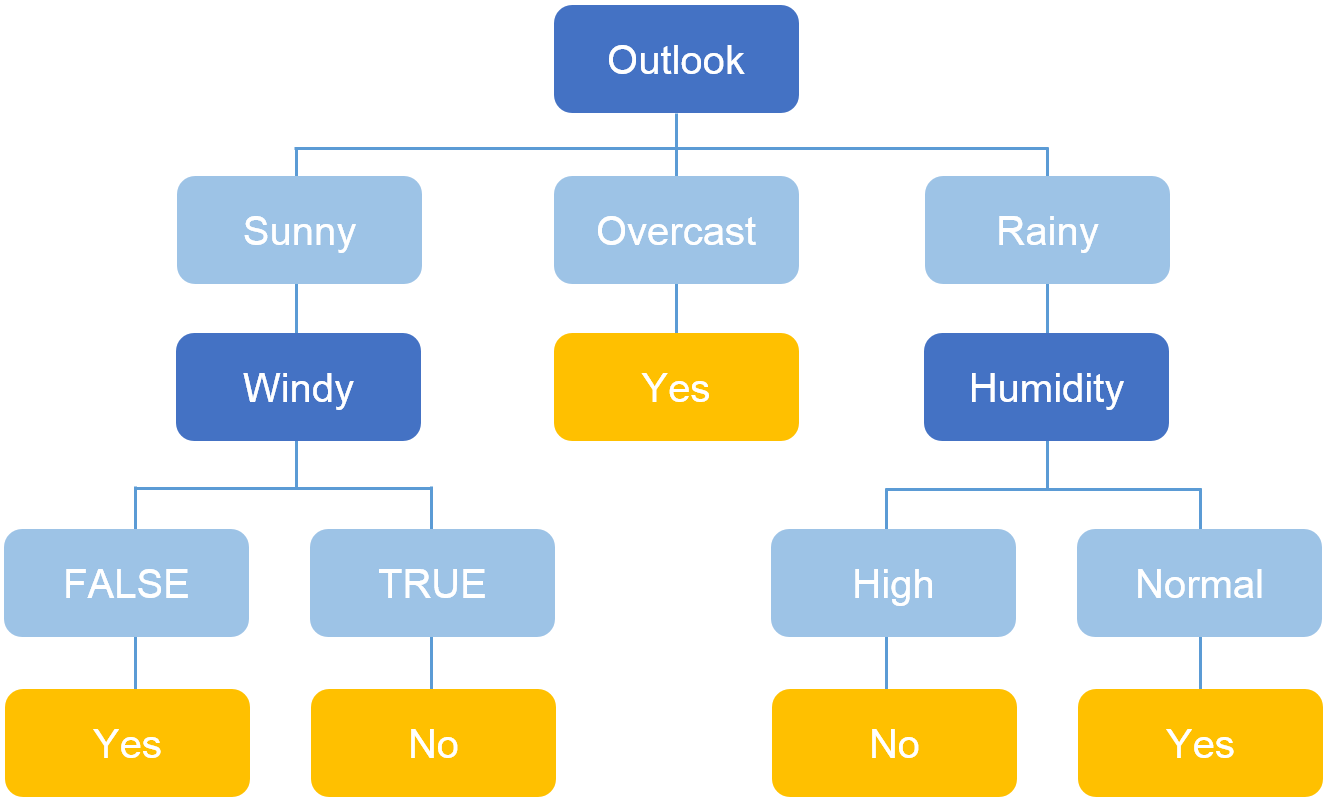
\includegraphics[width=0.26\linewidth]{img/dt.png}
	}
	\subfigure[SVM]{
		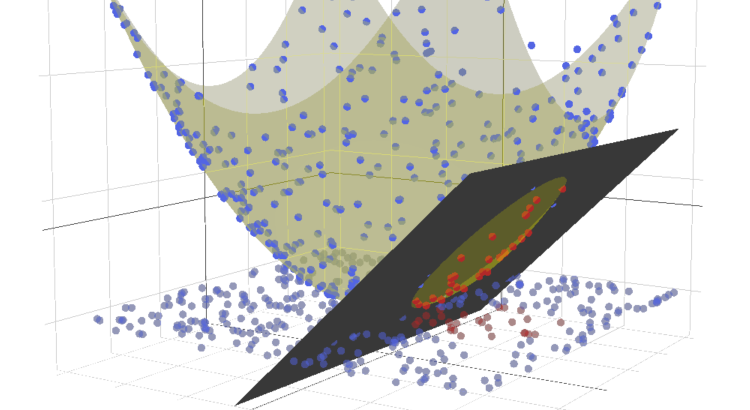
\includegraphics[width=0.28\linewidth]{img/svm.png}
	}
	\subfigure[MLP]{
		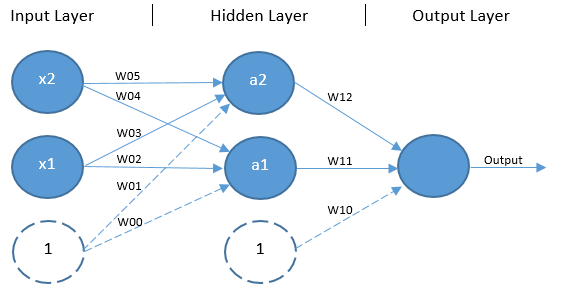
\includegraphics[width=0.28\linewidth]{img/mlp.png}
	}
	\caption{决策树、SVM和MLP模型的直观表示}
	\label{fig:model-init}
\end{figure}

\subsection{数据预处理}

在进行正式的分类之前,我对Adult数据集的特征和分类目标进行了一些预处理,以方便分类模型的训练。

\subsubsection{Z-score标准化(规范化)}

一般地,Z-score标准化有如下形式:
\begin{equation}
	y = \dfrac{x - \mu}{\sigma}
\end{equation}
其中$\mu$和$\sigma$分别代表原数据的均值和标准差。

\vspace{0.01\linewidth}
对于分类问题的数值型特征,经Z-score标准化后符合标准正态分布,即$N(0, 1)$,可以有效避免因数值过大导致的模型偏差,并能够加快模型的学习速率,这些优势在SVM和MLP等模型中表现得更加明显。

\vspace{0.01\linewidth}
除此之外,\ref{sec:num_feature}小节的结果表明,Adult数据集里的数值型特征大多近似服从正态分布,在这个条件下,Z-score标准化能够取得更良好的效果。若特征的分布与正态分布相差较大,则Z-score标准化反而会破坏原数据的分布,造成额外的偏差。

\subsubsection{向量化}

Adult数据集中存在8个类别型特征,且这些特征的类别之间并无大小关系,如性别的男女之间不存在大小的区别。为方便模型的训练,我将这些特征从字符串转化为one-hot向量。经过向量化处理后的数据,每个实例包含104维特征。

\subsubsection{分类目标修正}
\label{sec:fix-target}

Adult数据集的分类目标为居民收入,分为两类:<=50K\$以及>50K\$。而数据集中有些实例的分类目标后多了“.”,如变为“<=50K.”,直接使用原数据训练将导致分类目标变为4类。因此,我将分类目标转化为-1和1,分别表示<=50K\$和>50K\$。另外值得注意的一点是Adult数据集包含34014个负样本(<=50K),而仅有11208个正样本。

\subsection{分类性能评价标准}

对于分类问题,评价分类性能的标准一般有3个:精确度(precision),召回率(recall)以及f1-score。其在二分类问题中的定义如下。

假设二分类问题的结果为:


\begin{table}[H]
	\centering
	\begin{tabular}{c|c|c}
		& 正类 &  负类 \\
		\hline
		\hline
	
		 分类正确 & TP & FP \\
		 分类错误 & FN & TN \\
	\end{tabular}
\end{table}

则精确度、召回率和f1-score分别定义为
\begin{equation}
	\begin{aligned}
	P = \dfrac{TP}{TP + FP} \\ \\
	R = \dfrac{TP}{TP + FN} \\ \\
	F1 = \dfrac{2PR}{P + R} \\ \\
	\end{aligned}
\end{equation}

\vspace{-0.03\linewidth}
一般地,在大规模的数据集下,精确度和召回率会相互制约,出现一高一低的现象,而f1-score可以兼顾二者,有效减少因一者过大带来的误差。因此,在本次作业的实验中,我主要以\textbf{f1-score}作为分类性能的主要评价标准,精确度和召回率则在训练基线模型时作为参考标准。

\section{各分类模型的预测结果比较}
\label{sec:model-single}

\subsection{现有模型效果调查}

在开始训练分类模型前,我先调查了一些传统分类模型在Adult数据集上的分类效果 \cite{bench},衡量的标准为分类精确度,结果可参见表 \ref{tab:bench}。

\begin{table}[H]
	\centering
	\begin{tabular}{c|c}
		模型(算法) & 错误率(1-精确度) \\
		\hline
		\hline
	
		C4.5 & 15.54 \% \\
		C4.5-auto & 14.46 \% \\
		C4.5 rules & 14.94 \% \\
		Voted ID3 (0.6) & 15.64 \% \\
		Voted ID3 (0.8) & 16.47 \% \\
		T2 & 16.84 \% \\
		1R & 19.54 \% \\
		NBTree & 14.10 \% \\
		CN2 & 16.00 \% \\
		HOODG & 14.82 \% \\
		FSS Naive Bayes & 14.05 \% \\
		IDTM (Decision table) & 14.46 \% \\
		Naive-Bayes & 16.12 \% \\
		Nearest-neighbor (1) & 21.42 \% \\
		Nearest-neighbor (3) & 20.35 \% \\
		OC1 & 15.04 \% \\
		Pebls & 100 \% \\
		
	\end{tabular}
	\caption{传统分类模型在Adult数据集上的分类效果}
	\label{tab:bench}
\end{table}

\subsection{基线模型(baseline)}

为方便之后的比较,我首先使用sklearn \cite{sklearn}中的默认参数,不使用标准化,构造了三个基线模型,以及一个空模型(按相等概率 随机预测),参见表 \ref{tab:baselines1}和表 \ref{tab:baselines2}。

\begin{table}[H]
	\renewcommand\arraystretch{1.35}
	\caption{基线模型在Adult数据集上的性能(0.8-0.2比例的训练集-测试集分割)}
	\label{tab:baselines1}
	\centering
	
	\begin{tabular}{c|c|c|c|c}
		\centering
		 & 精确度(precision) & 召回率(recall) & f1-score & 时间(秒) \\
		\hline
		\hline
		
		决策树 & 0.81 & 0.81 & 0.81 & 0.25 \\
		SVM & 0.76 & 0.83 & 0.76 & 1044.22 \\
		MLP & 0.78 & 0.80 & 0.79 & 0.59 \\
		空模型 & 0.72 & 0.52 & 0.57 & 0.07 \\

	\end{tabular}
\end{table}

\begin{table}[H]
	\renewcommand\arraystretch{1.35}
	\caption{基线模型在Adult数据集上的性能(5折分层交叉验证)}
	\label{tab:baselines2}
	\centering
	
	\begin{tabular}{c|c|c|c|c}
		\centering
		 & 精确度(precision) & 召回率(recall) & f1-score & 时间(秒) \\
		\hline
		\hline
		
		决策树 & 0.80 & 0.80 & 0.80 & 4.41 \\
		SVM & 0.83 & 0.83 & 0.83 & 4491.21 \\
		MLP & 0.81 & 0.83 & 0.80 & 11.82 \\
		空模型 & 0.72 & 0.50 & 0.56 & 0.19 \\

	\end{tabular}
\end{table}

\subsection{决策树模型}

在本节中,我将使用网格搜索(Grid Search)对决策树模型的分类效果进行评估(5折交叉验证),搜索的参数及范围参见表 \ref{tab:dt-gs-para}。

\begin{table}[H]
	\renewcommand\arraystretch{1.35}
	\caption{对决策树模型网格搜索的参数及范围}
	\label{tab:dt-gs-para}
	\centering
	
	\begin{tabular}{c|c|c}
		\centering
		参数 & 含义 & 类型(范围) \\
		\hline
		\hline
		
		criterion & 特征选择的度量标准 & gini, entropy \\
		\hline
		max\_depth & 树的最大深度 & 正整数 \\
		\hline
		max\_features & \tabincell{c}{寻求最佳划分时\\要考虑的特征数目} & \tabincell{c}{总特征数或其平方根\\或其以2为底的对数值} \\
		\hline
		presort & 是否对数据预先排序 & 布尔值 \\
		\hline
		splitter & 结点划分策略 & best, random \\

	\end{tabular}
\end{table}

经过网格搜索后,我得到的最佳决策树模型的参数为:\{criterion: entropy, splitter: best, max\_features: 总特征数, max\_depth: 9, presort: True\};该模型在测试集上的平均f1-score为0.83。

对于经过Z-score标准化的Adult数据集,网格搜索的结果为:\{criterion: entropy, splitter: best, max\_features: 总特征数, max\_depth: 9, presort: True\},测试集上的平均f1-score为xxx。

\vspace{0.01\linewidth}
最终通过网格搜索筛选出的最佳决策树模型可视化见图 \ref{fig:dt-best-vis}。

\begin{figure}[H]
	\centering
	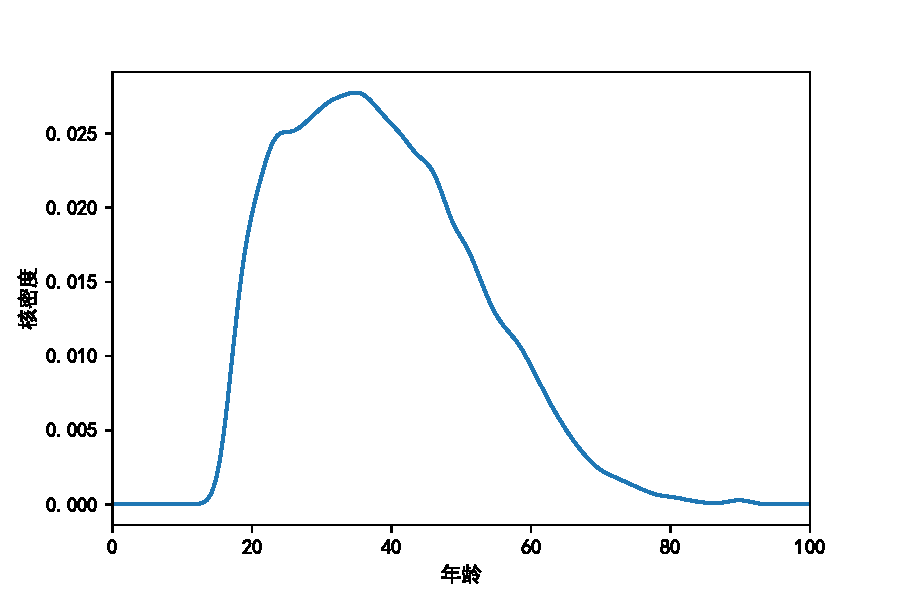
\includegraphics[width=0.9\linewidth]{img/age_dis.pdf}
	\caption{最佳决策树模型可视化}
	\label{fig:dt-best-vis}
\end{figure}

\subsection{SVM}

从表 \ref{tab:baselines1} 和表 \ref{tab:baselines2}来看,SVM的二分类能力并没有完全展现出来,并且难以收敛。在这一节中,我将尝试改变SVM模型的多个关键参数,尽可能改善其表现(模型表现均基于5折交叉验证)。

\subsubsection{核函数}

原始的SVM属于线性分类器,核函数的引入将SVM的应用推广到了非线性数据上。不同的核函数所需要的计算量和性能均有较大差别,我在Adult数据集上尝试应用四种常用的核函数:rbf核函数,多项式核函数(poly kernel),sigmoid核函数以及线性核函数,各模型相应的表现见图 \ref{fig:svm-kernel1} 及图 \ref{fig:svm-kernel2}。

\begin{figure}[H]
	\centering
	\subfigure[训练集]{
		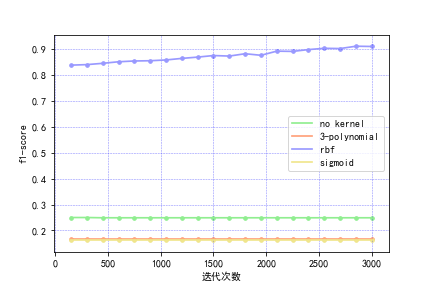
\includegraphics[width=0.41\linewidth]{img/svm_kernel_tr.png}
	}
	\subfigure[测试集]{
		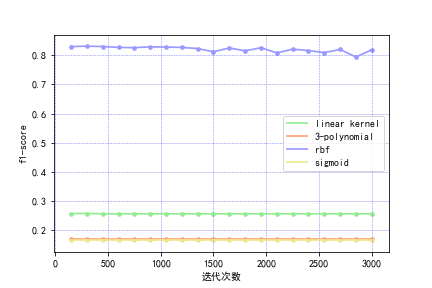
\includegraphics[width=0.41\linewidth]{img/svm_kernel_t.png}
	}
	\subfigure[训练集(标准化)]{
		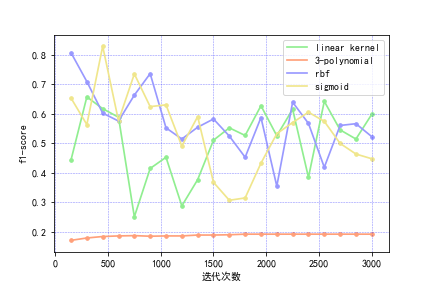
\includegraphics[width=0.41\linewidth]{img/svm_kernel_ntr.png}
	}
	\subfigure[测试集(标准化)]{
		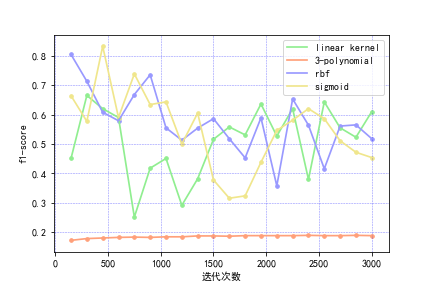
\includegraphics[width=0.41\linewidth]{img/svm_kernel_nt.png}
	}
	\caption{不同核函数下SVM模型的分类表现}
	\label{fig:svm-kernel1}
\end{figure}

\vspace{0.01\linewidth}
从上图中容易看出,对于未经Z-score标准化后的数据,SVM模型在使用rbf核时分类效果较佳,而其余核函数的分类效果极差,甚至低于空模型;而对于Z-score标准化后的数据,linear和sigmoid核函数的表现略有提高,但训练均极不稳定,向空模型的方向收敛。因此之后的实验均基于未Z-score标准化后的数据使用rbf核进行。

\subsubsection{惩罚系数}
\label{sec:penalty}

SVM在面对轻微的线性不可分数据时,可以通过引入惩罚系数$C$,将原有的优化目标
\begin{equation}
	L = \dfrac{1}{2}w^Tw
\end{equation}
变为
\begin{equation}
	L = \dfrac{1}{2}w^Tw+C\sum\limits_{n=1}^{N}\xi_n,
\end{equation}

适当的惩罚系数可以极大地改善SVM的分类性能。我使用类似于网格搜索的方式,遍历了各数量级的$C$取值,相应的结果可参见图 \ref{fig:penalty}。

\begin{figure}[H]
	\centering
	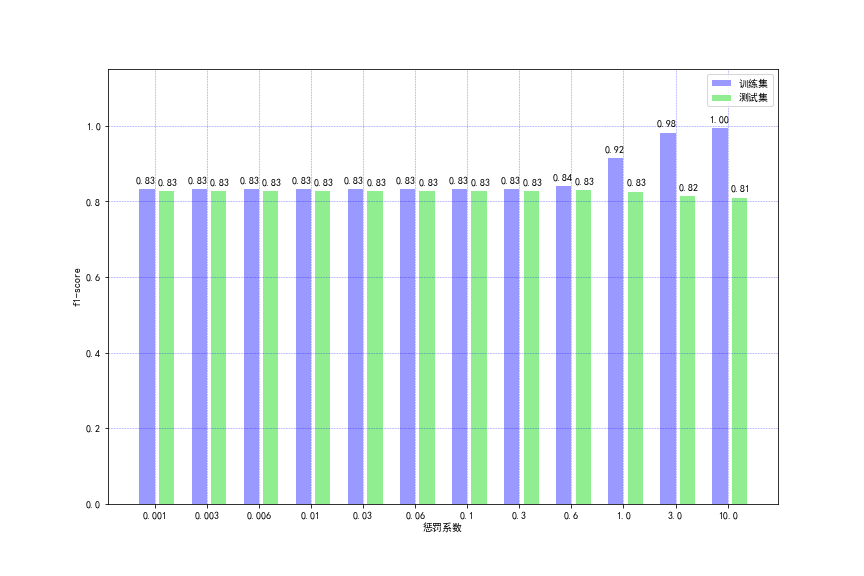
\includegraphics[width=0.75\linewidth]{img/svm_penalty.png}
	\caption{不同惩罚系数下SVM模型的分类表现}
	\label{fig:penalty}
\end{figure}

上图结果表明,过低的惩罚系数$C$对SVM在Adult数据集上的分类性能没有改善作用,0.6-1.0之间的$C$能够略微改善SVM的性能,而过大的$C$会让SVM趋于过拟合,泛化能力逐渐降低。

\subsubsection{Gamma ($\gamma$)}

rbf核的数学表达形式为:

\begin{equation}
	K(x_i, x_j)=exp(-\gamma\|x_i-x_j\|^2), \gamma>0
\end{equation}

$\gamma$是rbf核函数的一个重要参数,在sklearn中,其默认值为:$\dfrac{1}{\mbox{特征总维数}}$,在Adult数据集上即为$1/104=0.096$。我利用类似网格搜索的方式探索了各数量级下的$\gamma$对应的SVM模型的分类表现(表 \ref{tab:gammma})。

\begin{table}[H]
	\renewcommand\arraystretch{1.35}
	\caption{不同数量级的$\gamma$对应的SVM模型的分类表现}
	\label{tab:gammma}
	\centering
	
	\begin{tabular}{c|c|c}
		\centering
		$\gamma$ & 训练集f1-score & 测试集f1-score \\
		\hline
		\hline
		

	\end{tabular}
\end{table}

\subsubsection{小结}

经过以上的探索,我得到了SVM模型在Adult数据集分类上表现较佳的一组参数:\{核函数:rbf,惩罚参数:1.0,$\gamma$:xxx,是否进行Z-score标准化:否\},相应的SVM模型在测试集上的f1-score为:xxx。

\subsection{MLP}

从MLP基线模型(表 \ref{tab:baselines1}, \ref{tab:baselines2})的性能分析,MLP的性能相比决策树模型稍逊。我认为较大的原因在于MLP模型的默认参数并不适合Adult数据集,因此,在本节中,我将对MLP中不同的组件(激活函数,优化算法等)对其在Adult数据集上分类性能的影响进行探究。

\subsubsection{激活函数}

激活函数作用于MLP隐藏层中的每个神经元上,为MLP引入非线性因素,若缺少激活函数,神经网络的表达能力将极其有限。因此,激活函数是整个MLP中重要的组件之一。常用的激活函数包括relu \cite{{relu}}, tanh以及sigmoid等,相应的预测表现见图 \ref{fig:mlp-activate1}。

\begin{figure}[H]
	\centering
	\subfigure[训练集]{
		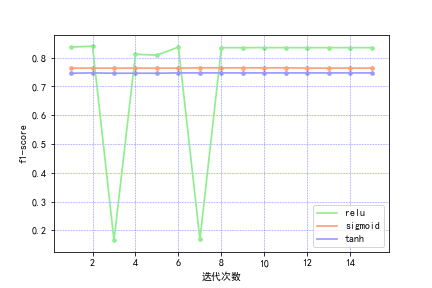
\includegraphics[width=0.41\linewidth]{img/mlp_activation_tr.png}
	}
	\subfigure[测试集]{
		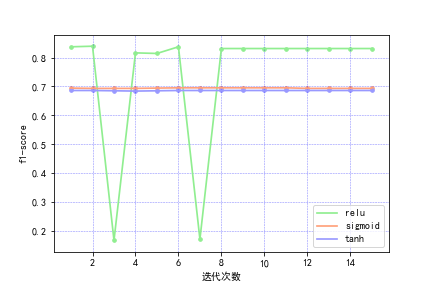
\includegraphics[width=0.41\linewidth]{img/mlp_activation_t.png}
	}
	\subfigure[训练集(标准化)]{
		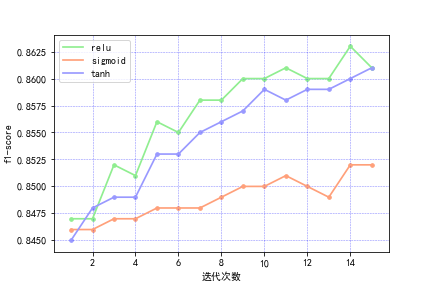
\includegraphics[width=0.41\linewidth]{img/mlp_activation_ntr.png}
	}
	\subfigure[测试集(标准化)]{
		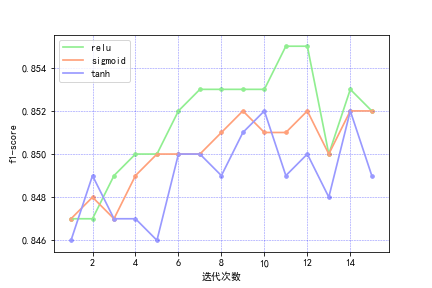
\includegraphics[width=0.41\linewidth]{img/mlp_activation_nt.png}
	}
	\caption{不同激活函数下MLP模型的分类表现}
	\label{fig:mlp-activate1}
\end{figure}

上图结果表明,相比于sigmoid和tanh,relu激活函数在Adult数据集下的分类表现更佳。同时,MLP在经过Z-score标准化后的Adult数据集上能取得更好的分类效果,不仅提高了整体的分类f1-score,更有效地避免了使用relu激活函数时进入局部最小值的情况。因此,之后MLP部分的实验均基于Z-score标准化后的Adult数据集进行。

\subsubsection{优化算法}

优化算法作用于MLP更新参数时,对于同样的梯度分布,不同的优化算法的优化路径存在着极大的差别,图 \ref{fig:optim-ref} 形象地说明了这一点。因此,探究不同优化算法下MLP的分类性能是很有必要的,详细结果可参见图 \ref{fig:optim1}。

\begin{figure}[H]
	\centering
	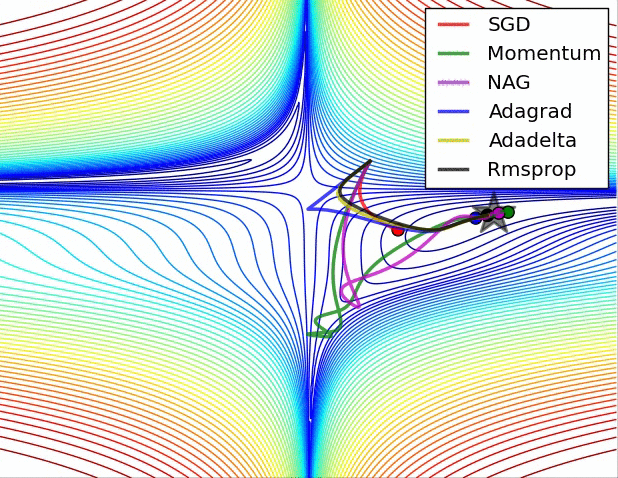
\includegraphics[width=0.5\linewidth]{img/optim_example.png}
	\caption{不同优化算法的优化效果对比 \cite{optim_example}}
	\label{fig:optim-ref}
\end{figure}

\begin{figure}[H]
	\centering
	\subfigure[训练集(标准化)]{
		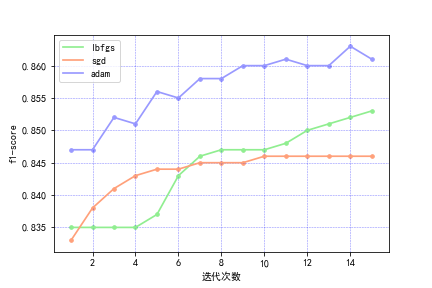
\includegraphics[width=0.41\linewidth]{img/mlp_optimizer_ntr.png}
	}
	\subfigure[测试集(标准化)]{
		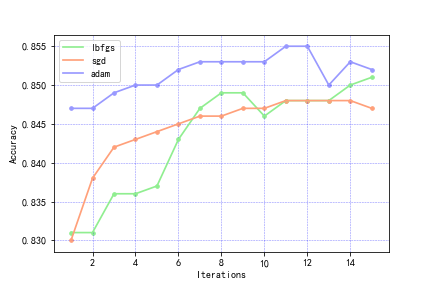
\includegraphics[width=0.41\linewidth]{img/mlp_optimizer_nt.png}
	}
	\caption{不同优化算法下MLP模型的分类表现}
	\label{fig:optim1}
\end{figure}

根据上图结果,adam \cite{adam}、lbfgs与sgd三种优化算法均能使MLP在Adult数据集上取得较佳的分类表现,但adam的效果明显优于lbfgs与sgd,为探究其中的原因,我查阅了相关资料和原论文,认为图中反映出adam算法的巨大优势有着其坚实的理论依据。

\vspace{0.01\linewidth}
作为最常用的优化算法,adam能够利用较少的计算资源有效处理高噪声或稀疏的梯度分布,除此之外,其在优化的过程中能够通过计算梯度的一阶矩估计和二阶矩估计,为不同的参数设计独立的自适应性学习率。

\subsubsection{学习率}

在MLP的参数更新过程中,学习率决定了参数更新的速率,过大的学习率会导致模型进入局部最小值,而学习率过小则会减缓模型的学习速度。在本节中,我采用类似于 \ref{sec:penalty}小节的方式,对基于adam优化算法的MLP模型在不同学习率下的分类效果进行探索(图 \ref{fig:lr}),由于adam算法能够自适应地改变学习率,此处的学习率即指\textbf{初始学习率}。

\begin{figure}[H]
	\centering
	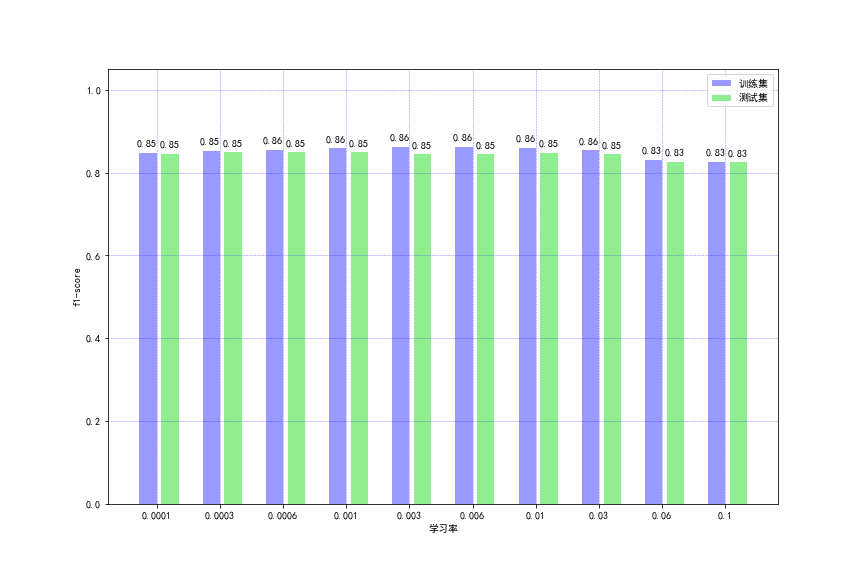
\includegraphics[width=0.75\linewidth]{img/mlp_lr.png}
	\caption{不同初始学习率下MLP模型的分类表现}
	\label{fig:lr}
\end{figure}

容易看出,除了过大的学习率有降低MLP性能的趋势外,MLP在其余学习率下的表现并无太大差别,考虑到实际应用时的时间占用,我认为0.03是基于adam优化算法的MLP模型在Adult数据集分类问题下较佳的学习率。

\subsubsection{小结}

经过以上的探索,我得到了MLP模型在Adult数据集分类上表现较佳的一组参数:\{激活函数:relu,优化算法:adam,学习率:0.03,是否进行Z-score标准化:是\},相应的MLP模型在测试集上的f1-score为:xxx。

\subsection{模型集成}

从以上几节的结果分析,决策树模型在Adult数据集上的分类效果弱于SVM和MLP。一般地,从一系列模型$M_1, M_2, ... , M_k$创建组合模型$M^*$,可以有效提高原模型的效果。相比于SVM和MLP,决策树模型训练时速度快、占用计算空间和资源较少,适合进行模型集成。

\vspace{0.01\linewidth}
因此,在本节中,我使用bagging和boosting两种模型集成的方法尝试改善决策树模型的分类效果。结果参见图 \ref{fig:model-plus}。

\begin{figure}[H]
	\centering
	\subfigure[bagging]{
		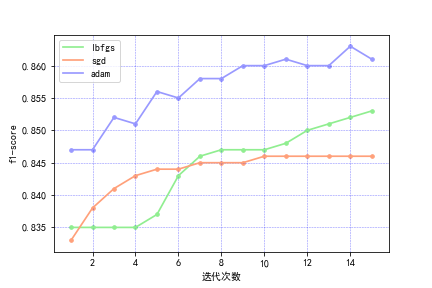
\includegraphics[width=0.31\linewidth]{img/mlp_optimizer_ntr.png}
	}
	\subfigure[boosting(SAMME)]{
		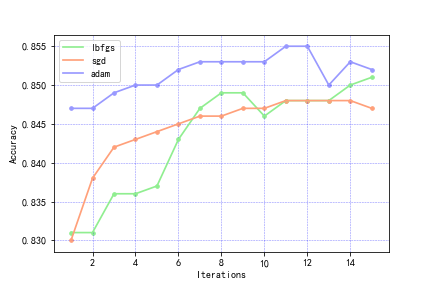
\includegraphics[width=0.31\linewidth]{img/mlp_optimizer_nt.png}
	}
	\subfigure[boosting(SAMME.R)]{
		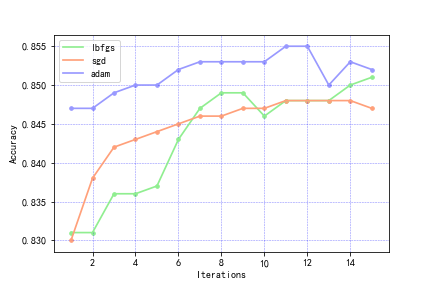
\includegraphics[width=0.31\linewidth]{img/mlp_optimizer_nt.png}
	}
	\caption{集成后的决策树模型的分类表现}
	\label{fig:model-plus}
\end{figure}

\subsection{三种分类模型效果对比}
\label{sec:compare}

通过第 \ref{sec:model-single}小节的实验,我对决策树、SVM和MLP三种模型在Adult数据集上的分类效果有了大致的了解。在本节中,我将探索三种分类模型在不同条件下对Adult数据集的分类效果。

\subsubsection{Z-score标准化}

在前文的探索过程中,我已分别得到了三种模型在Z-score标准化前后的数据上的分类表现,在本节中我将这些结果进行一个直观的表示,方便观察在Adult数据集下,Z-score标准化对于三种模型的适合程度,如表 \ref{tab:norm}。

\begin{table}[H]
	\renewcommand\arraystretch{1.35}
	\caption{三种分类模型在Z-score标准化前后的数据上的分类表现}
	\label{tab:norm}
	\centering
	
	\begin{tabular}{c|c|c}
		\centering
		 & 测试集f1-score(标准化前) & 测试集f1-score(标准化后) \\
		\hline
		\hline
		
		决策树 & & \\
		SVM & & \\
		MLP & & \\	

	\end{tabular}
\end{table}

\subsubsection{PCA}

从 \ref{sec:cof}小节的结果可知,Adult数据集的特征之间存在一定的相关性,即可能存在冗余的特征,因此我在本小节中对原数据进行PCA降维,并探索三种分类模型在降维后数据上的分类表现(图 \ref{fig:pca1})。

\begin{figure}[H]
	\centering
	\subfigure[bagging]{
		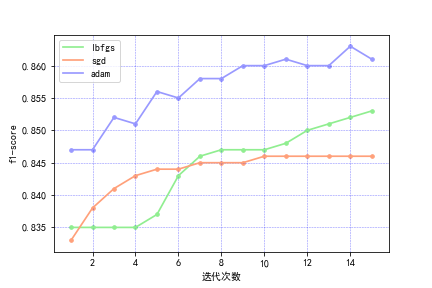
\includegraphics[width=0.31\linewidth]{img/mlp_optimizer_ntr.png}
	}
	\subfigure[boosting(SAMME)]{
		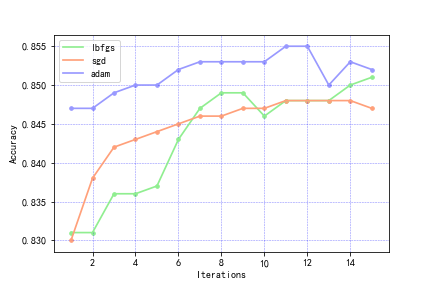
\includegraphics[width=0.31\linewidth]{img/mlp_optimizer_nt.png}
	}
	\subfigure[boosting(SAMME.R)]{
		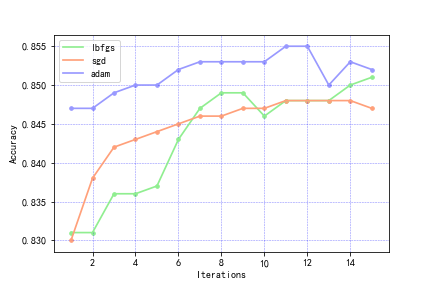
\includegraphics[width=0.31\linewidth]{img/mlp_optimizer_nt.png}
	}
	\caption{决策树、SVM和MLP在降维后数据上的分类表现}
	\label{fig:pca1}
\end{figure}

\subsubsection{最佳性能对比}

根据 \ref{sec:model-single} 与 \ref{sec:compare}小节的实验结果,三种模型均存在一个最佳的f1-score值,一定程度上代表其在Adult数据集上分类能力的极限(由于模型的参数空间极其巨大,无法保证该值是否为全局最优,但在一定程度上能反映该模型的最佳性能),对比参见表 \ref{tab:final_compare}。

\begin{table}[H]
	\renewcommand\arraystretch{1.35}
	\caption{三种分类模型在Adult数据集下的最佳分类性能}
	\label{tab:final_compare}
	\centering
	
	\begin{tabular}{c|c|c}
		\centering
		 & 训练集f1-score & 测试集f1-score \\
		\hline
		\hline
		
		决策树 & & \\
		SVM & & \\
		MLP & & \\	

	\end{tabular}
\end{table}

%\begin{figure}[H]
%	\centering
%	\subfigure[决策树]{
%		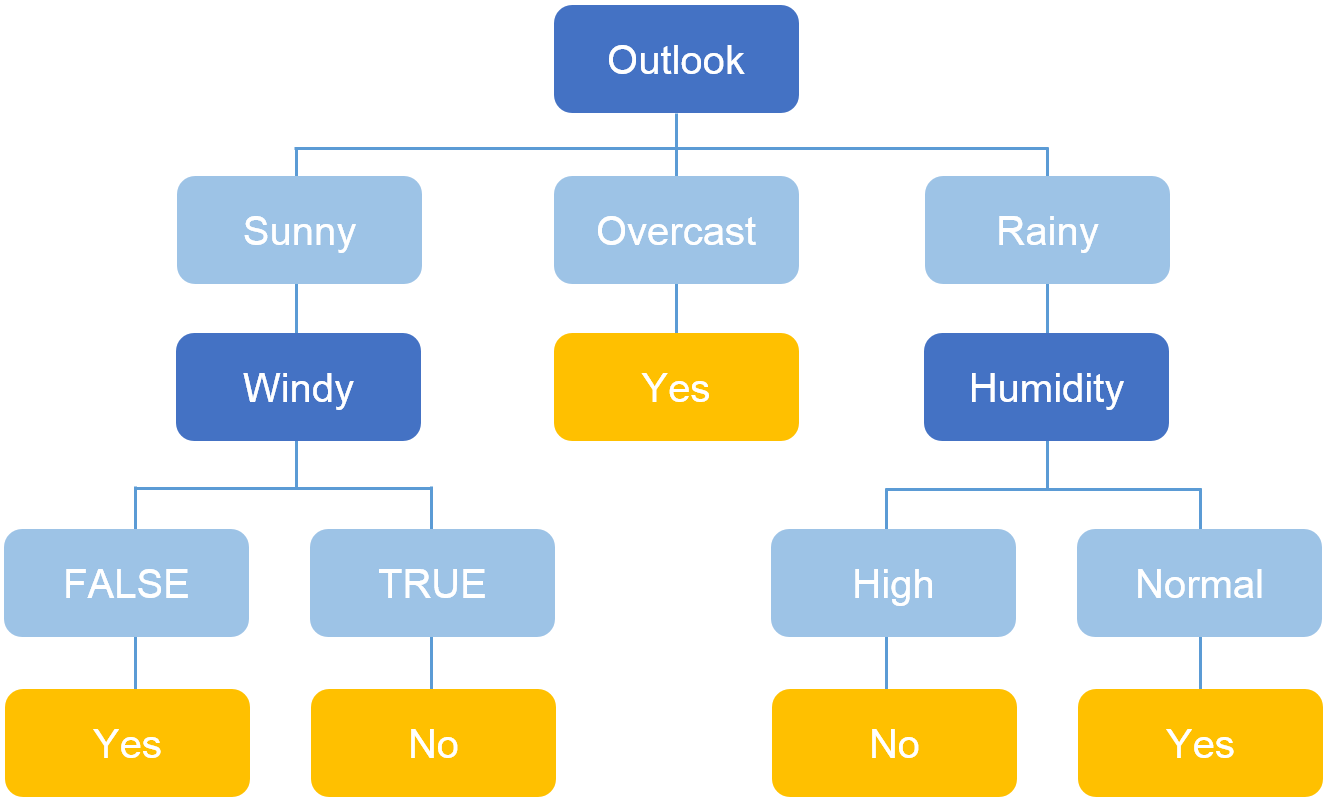
\includegraphics[width=0.23\linewidth]{img/dt.png}
%	}
%	\subfigure[SVM]{
%		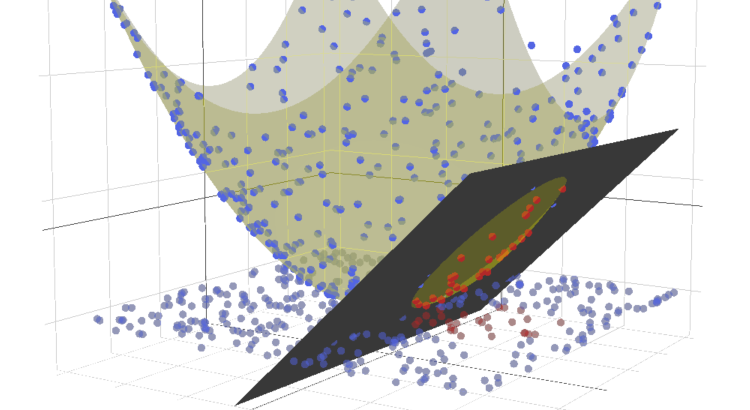
\includegraphics[width=0.23\linewidth]{img/svm.png}
%	}
%	\subfigure[MLP]{
%		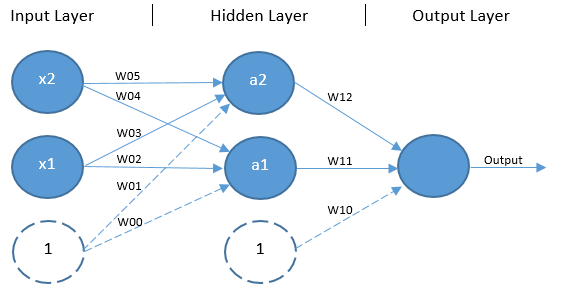
\includegraphics[width=0.23\linewidth]{img/mlp.png}
%	}
%	\subfigure[空模型]{
%		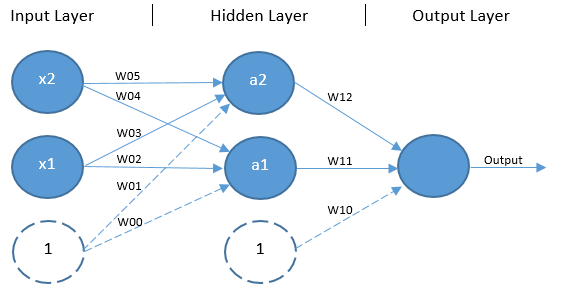
\includegraphics[width=0.23\linewidth]{img/mlp.png}
%	}
%	\subfigure[决策树]{
%		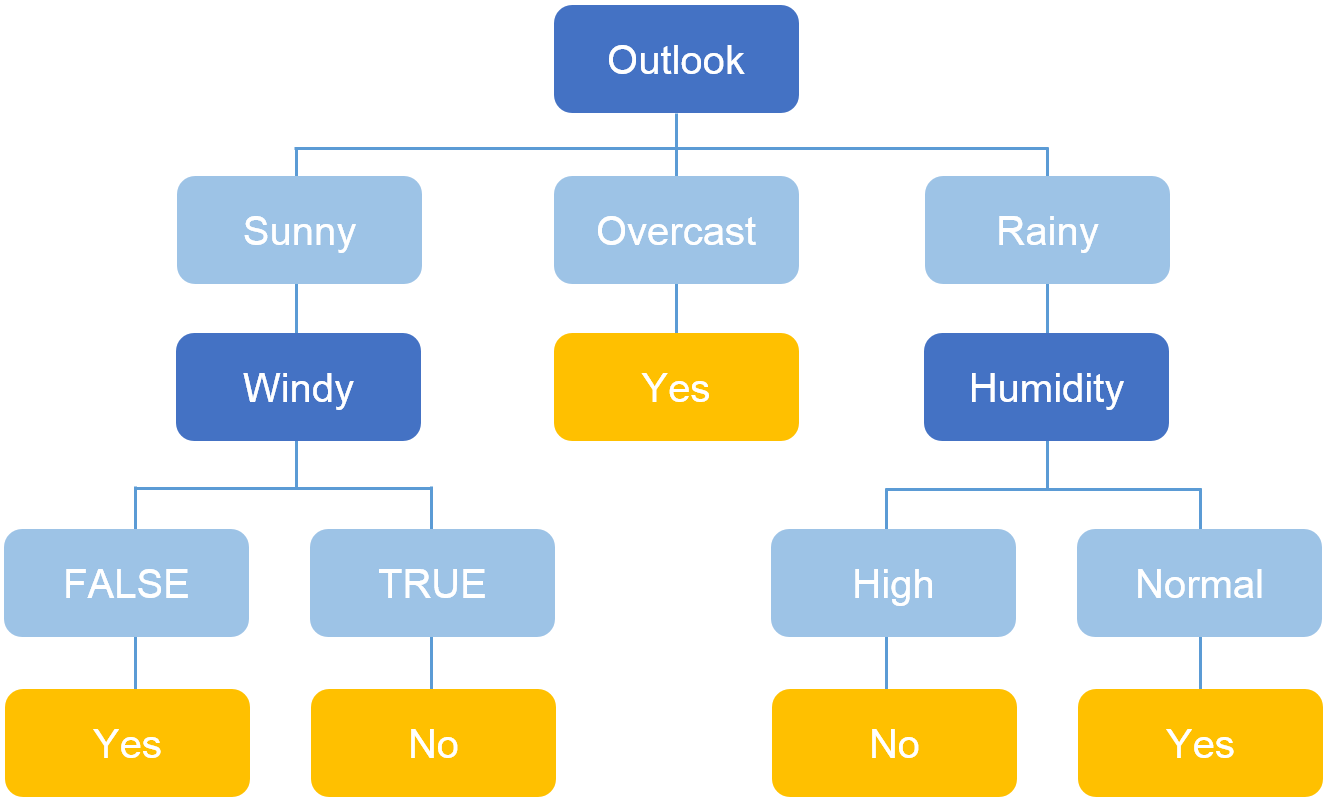
\includegraphics[width=0.23\linewidth]{img/dt.png}
%	}
%	\subfigure[SVM]{
%		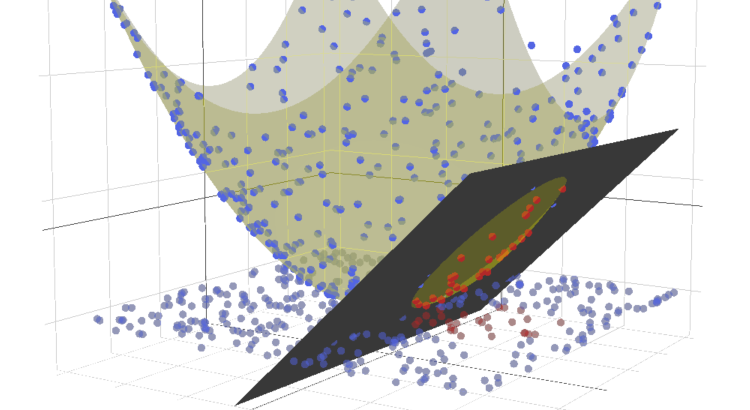
\includegraphics[width=0.23\linewidth]{img/svm.png}
%	}
%	\subfigure[MLP]{
%		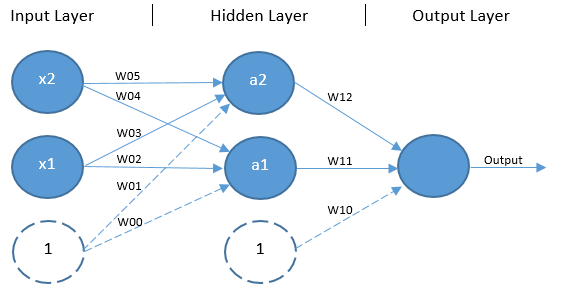
\includegraphics[width=0.23\linewidth]{img/mlp.png}
%	}
%	\subfigure[空模型]{
%		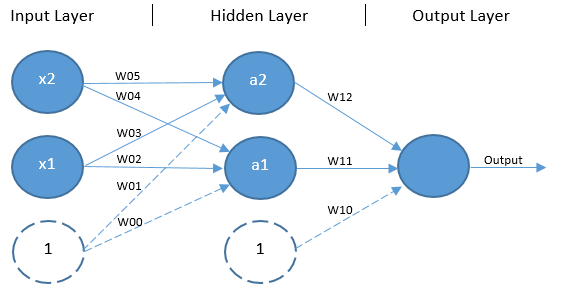
\includegraphics[width=0.23\linewidth]{img/mlp.png}
%	}
%	\subfigure[决策树]{
%		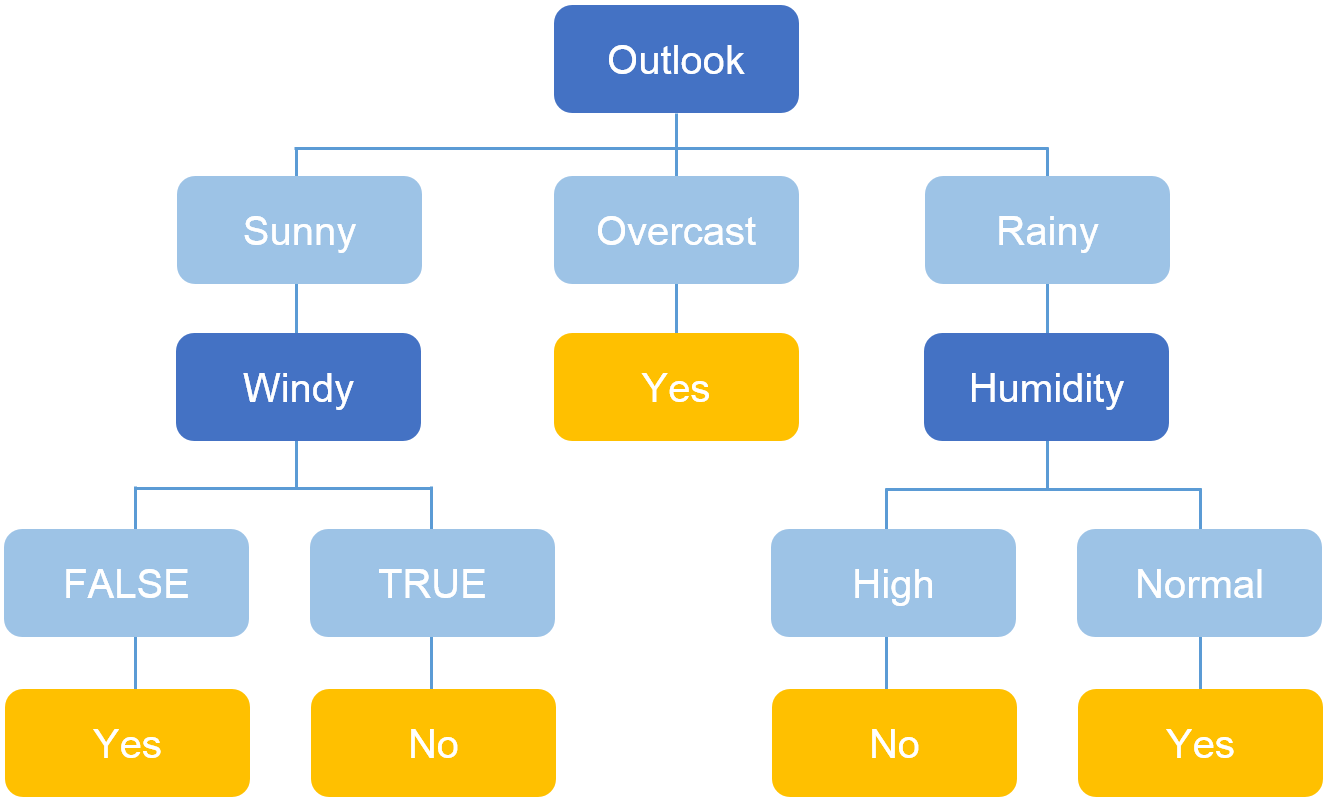
\includegraphics[width=0.23\linewidth]{img/dt.png}
%	}
%	\subfigure[SVM]{
%		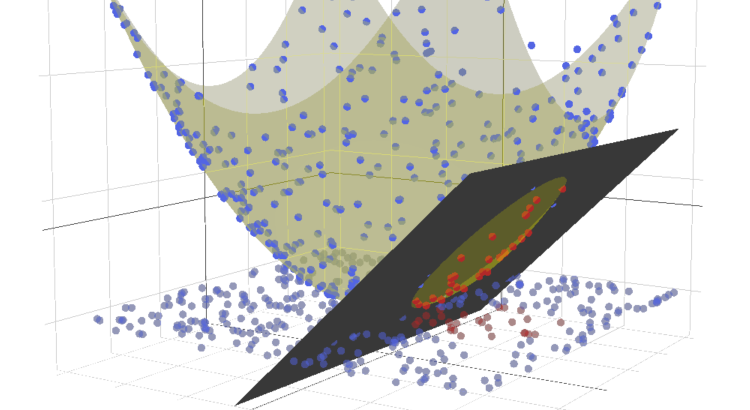
\includegraphics[width=0.23\linewidth]{img/svm.png}
%	}
%	\subfigure[MLP]{
%		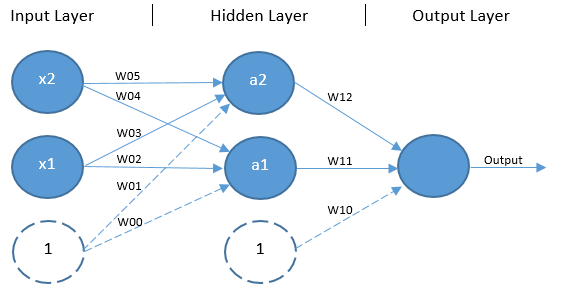
\includegraphics[width=0.23\linewidth]{img/mlp.png}
%	}
%	\subfigure[空模型]{
%		\includegraphics[width=0.23\linewidth]{img/mlp.png}
%	}
%	\caption{基线模型(第一、二行的数据集划分分别为0.8-0.2,以及0.7-0.3的训练集-测试集划分,第三行则使用了5折分层交叉验证}
%	\label{fig:baselines}
%\end{figure}

\section{对Adult数据集的分析结论}

Adult数据集是一个中等规模,存在少部分缺失值的二分类数据集,共48842个实例,每个实例包含14个特征,其中8个为类别型特征,6个为数值型特征。各类别型特征的分布差异较大,数值型特征的分布近似于正态分布。

\vspace{0.01\linewidth}
我使用了决策树、SVM和MLP三种分类模型对Adult数据集进行分类,对模型的参数进行微调后,xxx的分类效果最佳,最高的f1-score可达到xxx,而xxx模型所消耗的时间最少,平均不到xxx秒。除使用单独模型进行分类外,我还对决策树模型进行了模型集成(bagging和boosting),集成后的模型xxx。


\newpage
\begin{appendix}
	\section{附录}
	\subsection{作业中使用的工具及库包}
	\label{apd:tools}
	本次作业我所使用的编程语言为Python \cite{python},编辑环境以jupyter notebook \cite{notebook} 为主。作业中我使用的库包见表 \ref{tab:import}。
	
	\begin{table}[H]
		\renewcommand\arraystretch{1.35}
		\caption{本作业中使用的库包}
		\label{tab:import}
		\centering
		
		\begin{tabular}{c|c}
			\centering
			库包名 &  用途 \\
			\hline
	
			numpy \cite{numpy} & 处理数据,数值计算 \\
			pandas \cite{pandas} & 读取数据,绘图,处理数据 \\
			matplotlib \cite{matplotlib} & 绘图 \\
			scipy \cite{scipy} & 数值计算 \\
			scikit-learn \cite{sklearn} & 分类模型的构造和运算 \\
	
		\end{tabular}
	\end{table}
	
	\subsection{Adult数据集特征分布补充资料}
	
	\subsubsection{Adult数据集所有属性分布直方图}
	\label{apd:attri}
	
	\vspace{-0.02\linewidth}
	\begin{figure}[H]
		\centering
		\includegraphics[width=0.75\linewidth]{img/native_country_dis2.pdf}
		\caption{Adult数据集native-country特征分布(除United-States)}
		\label{fig:attri_detail}
	\end{figure}
	
	\subsubsection{native-country特征的详细分布}
	\label{apd:native-country}
	
	\vspace{-0.02\linewidth}
	\begin{figure}[H]
		\centering
		\includegraphics[width=0.75\linewidth]{img/native_country_dis2.pdf}
		\caption{Adult数据集native-country特征分布(除United-States)}
		\label{fig:class_feature_dis_detail}
	\end{figure}
	
	\subsubsection{各类别型特征下的详细类名}
	\label{apd:classes}
	
	\begin{enumerate}
	
	\item \textbf{workclass} Private, Local-gov, Self-emp-not-inc, Federal-gov, State-gov, Self-emp-inc, Without-pay, Never-worked;
	
	\item \textbf{education} 11th, HS-grad, Assoc-acdm, Some-college, 10th, Prof-school, 7th-8th, Bachelors, Masters, Doctorate, 5th-6th, Assoc-voc, 9th, 12th, 1st-4th, Preschool;
	
	\item \textbf{marital-status} Never-married, Married-civ-spouse, Widowed, Divorced, Separated, Married-spouse-absent, Married-AF-spouse;
	
	\item \textbf{occupation} Machine-op-inspct, Farming-fishing, Protective-serv, Other-service, Prof-specialty, Craft-repair, Adm-clerical, Exec-managerial, Tech-support, Sales, Priv-house-serv, Transport-moving, Handlers-cleaners, Armed-Forces;
	
	\item \textbf{relationship} Own-child, Husband, Not-in-family, Unmarried, Wife, Other-relative;
	
	\item \textbf{race} Black, White, Asian-Pac-Islander, Other, Amer-Indian-Eskimo;
	
	\item \textbf{sex} Male, Female;
	
	\item \textbf{native-country} United-States, Cuba, Jamaica, India, Mexico, Puerto-Rico, Honduras, England, Canada, Germany, Iran, Philippines, Poland, Columbia, Cambodia, Thailand, Ecuador, Laos, Taiwan, Haiti, Portugal, Dominican-Republic, El-Salvador, France, Guatemala, Italy, China, South, Japan, Yugoslavia, Peru, Outlying-US(Guam-USVI-etc), Scotland, Trinadad\&Tobago, Greece, Nicaragua, Vietnam, Hong, Ireland, Hungary, Holand-Netherlands.
	       
	\end{enumerate}
	
\end{appendix}

\bibliographystyle{ieeetr}
\bibliography{bio}

%========================================================================
\end{document}